\documentclass[bachelor, och, coursework]{SCWorks}
% параметр - тип обучения - одно из значений:
%    spec     - специальность
%    bachelor - бакалавриат (по умолчанию)
%    master   - магистратура
% параметр - форма обучения - одно из значений:
%    och   - очное (по умолчанию)
%    zaoch - заочное
% параметр - тип работы - одно из значений:
%    referat    - реферат
%    coursework - курсовая работа (по умолчанию)
%    diploma    - дипломная работа
%    pract      - отчет по практике
% параметр - включение шрифта
%    times    - включение шрифта Times New Roman (если установлен)
%               по умолчанию выключен
\usepackage{subfigure}
\usepackage{tikz,pgfplots}
\pgfplotsset{compat=1.5}
\usepackage{float}

%\usepackage{titlesec}
\setcounter{secnumdepth}{4}
%\titleformat{\paragraph}
%{\normalfont\normalsize}{\theparagraph}{1em}{}
%\titlespacing*{\paragraph}
%{35.5pt}{3.25ex plus 1ex minus .2ex}{1.5ex plus .2ex}

\titleformat{\paragraph}[block]
{\hspace{1.25cm}\normalfont}
{\theparagraph}{1ex}{}
\titlespacing{\paragraph}
{0cm}{2ex plus 1ex minus .2ex}{.4ex plus.2ex}

% --------------------------------------------------------------------------%


\usepackage[T2A]{fontenc}
\usepackage[utf8]{inputenc}
\usepackage{graphicx}
\graphicspath{ {./images/} }
\usepackage{tempora}

\usepackage[sort,compress]{cite}
\usepackage{amsmath}
\usepackage{amssymb}
\usepackage{amsthm}
\usepackage{fancyvrb}
\usepackage{listings}
\usepackage{listingsutf8}
\usepackage{longtable}
\usepackage{array}
\usepackage[english,russian]{babel}

% \usepackage[colorlinks=true]{hyperref}
\usepackage{url}

\usepackage{underscore}
\usepackage{setspace}
\usepackage{indentfirst} 
\usepackage{mathtools}
\usepackage{amsfonts}
\usepackage{enumitem}
\usepackage{tikz}
\usepackage{minted}

\newcommand{\eqdef}{\stackrel {\rm def}{=}}
\newcommand{\specialcell}[2][c]{%
\begin{tabular}[#1]{@{}c@{}}#2\end{tabular}}

\renewcommand\theFancyVerbLine{\small\arabic{FancyVerbLine}}

\newtheorem{lem}{Лемма}

\begin{document}

% Кафедра (в родительном падеже)
\chair{теоретических основ компьютерной безопасности и криптографии}

% Тема работы
\title{Обнаружение сетевого RDP трафика методом анализа его поведения}

% Курс
\course{3}

% Группа
\group{331}

% Факультет (в родительном падеже) (по умолчанию "факультета КНиИТ")
\department{факультета КНиИТ}

% Специальность/направление код - наименование
%\napravlenie{09.03.04 "--- Программная инженерия}
%\napravlenie{010500 "--- Математическое обеспечение и администрирование информационных систем}
%\napravlenie{230100 "--- Информатика и вычислительная техника}
%\napravlenie{231000 "--- Программная инженерия}
\napravlenie{10.05.01 "--- Компьютерная безопасность}

% Для студентки. Для работы студента следующая команда не нужна.
% \studenttitle{Студентки}

% Фамилия, имя, отчество в родительном падеже
\author{Токарева Никиты Сергеевича}

% Заведующий кафедрой
\chtitle{} % степень, звание
\chname{Абросимов М. Б.}

%Научный руководитель (для реферата преподаватель проверяющий работу)
\satitle{доцент} %должность, степень, звание
\saname{Гортинский А. В.}

% Руководитель практики от организации (только для практики,
% для остальных типов работ не используется)
% \patitle{к.ф.-м.н.}
% \paname{С.~В.~Миронов}

% Семестр (только для практики, для остальных
% типов работ не используется)
%\term{8}

% Наименование практики (только для практики, для остальных
% типов работ не используется)
%\practtype{преддипломная}

% Продолжительность практики (количество недель) (только для практики,
% для остальных типов работ не используется)
%\duration{4}

% Даты начала и окончания практики (только для практики, для остальных
% типов работ не используется)
%\practStart{30.04.2019}
%\practFinish{27.05.2019}

% Год выполнения отчета
\date{2022}

\maketitle

% Включение нумерации рисунков, формул и таблиц по разделам
% (по умолчанию - нумерация сквозная)
% (допускается оба вида нумерации)
% \secNumbering

%-------------------------------------------------------------------------------------------

\tableofcontents

\intro
Информация -- это сведения об окружающем мире и протекающих в нём процессах, которые зафиксированы на каком-либо носителе.
Благодаря протоколам удаленного доступа можно распоряжаться базами данных, информацией, которая хранится на другом устройстве. В недавнем прошлом большинство
схем удаленного доступа характеризовалось высокой стоимостью, низкой производительностью, небольшой скоростью передачи данных, недостаточным уровнем защищенности
передаваемой информации \cite{1}. 

Сейчас, когда практически все предприятия перешли на дистанционный формат работы, компании выбирают протокол RDP, так как он прост в настройке и в использовании.
Но далеко не все уделяют особое внимание безопасности собственных рабочих мест. Поэтому предприятия могут быть атакованы злоумышленниками.

В данной работе будут разобраны принцип работы RDP, анализ его поведения, а также методы обнаружения данного протокола.

\section{Определение RDP}

Протокол RDP (от англ. Remote Desktop Protocol --- протокол удалённого рабочего стола) --- патентованный протокол 
прикладного уровня компании Microsoft и приобретен ею у другой компании Polycom, который предоставляет пользователю графический интерфейс для 
подключения к другому компьютеру через сетевое соединение. Для этого пользователь запускает клиентское программное обеспечение RDP, а на другом 
компьютере должно быть запущено программное обеспечение сервера RDP \cite{2}.

Клиенты для подключения по RDP существуют для большинства версий Microsoft Windows, Linux, Unix, macOS, iOS, Android и 
других операционных систем. Стоит отметить, что RDP-серверы встроены в операционные системы Windows. По умолчанию подключения, созданные с 
помощью RDP, используют UDP-порт 3389 и TCP порт 3389, по которым осуществляется передача данных.

\subsection{Безопасность протокола RDP}

Как уже известно, что для операционной системы Windows постоянно выходят различные обновления, включая обновлений RDS (от англ. Remote Desktop Services --- службы 
удаленных рабочих столов). В связи с этим возникают различные уязвимости при инициализации RDP-сессии. В основном они не связаны непосредственно с
протоколом RDP, но касаются службы удаленных рабочих столов RDS и позволяют при успешной эксплуатации путем отправления специального запроса через RDP
получить возможность выполнения произвольного кода на уязвимой системе, даже не проходя при этом процедуру проверки подлинности. Достаточно лишь иметь доступ
к хосту или серверу с уязвимой системой Windows. Таким образом, любая система, доступная из сети Интернет, является уязвимой при отсутствии установленных
последних обновлений безопасности Windows.

Если стоит задача защитить удаленный доступ, то, конечно, необходимо использовать надежный пароль, обновить свое программное обеспечение до последней версии,
также можно использовать VPN подключение, чтобы получить IP-адрес виртуальной сети и добавить его в правило исключения брандмауэра RDP. Стоит отметить, что
существует много разных способов, чтобы защитить подключение с помощью протокола RDP и более подробно это описано в документации Microsoft.

  \section{Принцип работы протокола RDP и анализ его поведения}

  Принцип работы RDP базируется на протоколе TCP. Соединение клиент-сервер происходит на транспортном уровне. После инициализации пользователь 
  проходит аутентификацию. В случае успешного подтверждения сервер передает клиенту управление. Стоит отметить, что под понятием слова <<клиент>> подразумевается
  любое устройство (персональный компьютер, планшет или смартфон), а <<сервер>> --- удаленный компьютер, к которому оно подключается.

  Протокол RDP внутри себя поддерживает виртуальные каналы, через которые пользователю передаются дополнительные функции операционной системы,
  например, можно распечатать документ, воспроизвести видео или скопировать файл в буфер обмена.

  % Известно, что RDP является прикладным протоколом, базирующимся на TCP. Для начала пользователю необходимо установить соединение клиент-сервер, которое
  % происходит на транспортном уровне. После инициализации RDP-сессии производится аутентификация. Далее сервер начинает передавать клиенту графический вывод и
  % ожидает входные данные от клавиатуры и мыши. В качестве графического вывода может выступать как точная копия графического экрана, передаваемая как изображение,
  % так и команды на отрисовку графических примитивов, например, линия, круг, эллипс, текст и др. Для протокола RDP приоритетом является передача вывода с помощью
  % примитивов, так как это экономит трафик. Изображение передается только в том случае, если не удалось согласовать параметры передачи примитивов при установке 
  % RDP-сессии. Обработка полученных команд и вывод изображения осуществляется с помощью графической подсистемы RDP-клинта. Сигнал нажатия и отпускания клавиши клавиатуры
  % шифруются и ожидают команды отправки \cite{3}.
  
  Далее в работе будет описан процесс установки RDP-сессии, во время которой осуществляется захват трафика с помощью одной известной программы Wireshark. С помощью нее
  можно достаточно подробно рассмотреть структуру сообщений протоколов.

  Для начала будет произведено подключение с помощью <<Удаленного рабочего стола>>. Это средство представляет собой встроенную в Windows программу, предназначенную
  для удалённого доступа. При его использовании предполагается, что пользователь будет подключаться к одному компьютеру с другого устройства, находящегося в той же
  локальной сети. В качестве клиента и сервера будут выступать компьютеры с операционной системой Windows 10 Professional версии 21H2. 
  
  Для подключения к удаленному рабочему столу были заданы статические IP-адреса. Клиенту был присвоен статический IP-адрес 192.168.10.254,
  а серверу --- 192.168.10.229, соответственно маска сети 255.255.255.0. После того, как были заданы IP-адреса, необходимо зайти в настройки
  Windows, чтобы включить возможность подключения к удаленному рабочему столу. Об этом более подробно описано
  в статьях \cite{userdp1} и \cite{userdp2}. Далее на сервере был произведен запуск анализа трафика с помощью приложения Wireshark.
  После подключения к удаленному компьютеру программа-анализатор трафика начала <<захватывать>> пакеты, как показано на рисунке \ref{wireshark1},
  принадлежащие следующим протоколам:
  
  \begin{figure}[H]
    \centering
    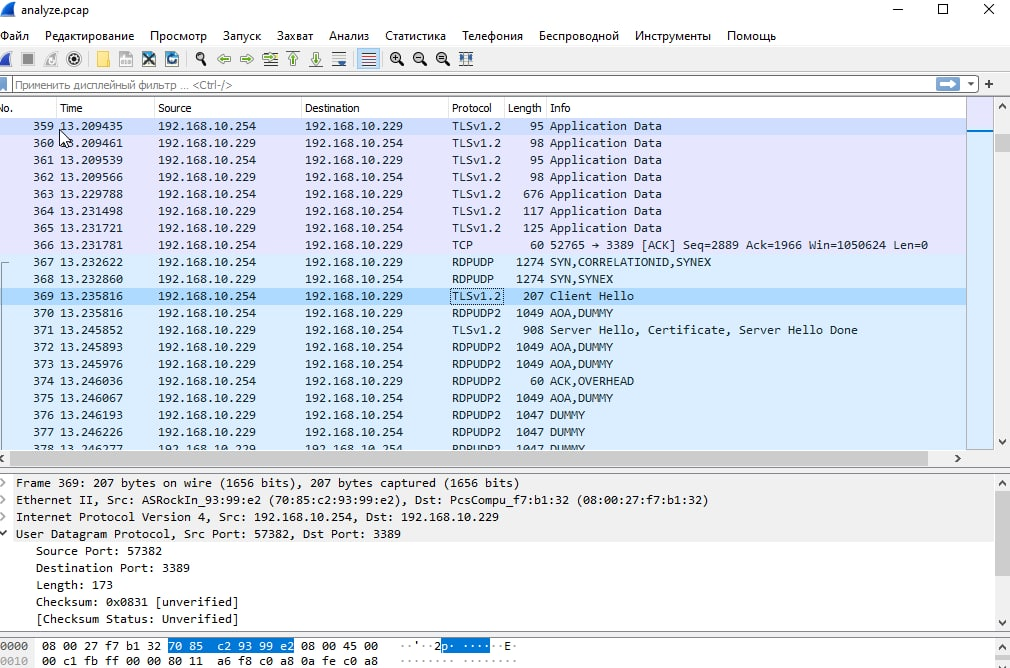
\includegraphics[width=0.8\textwidth]{photo/wireshark1.png}
    \caption{Окно программы Wireshark после захвата трафика}
    \label{wireshark1}
  \end{figure}

  \begin{itemize}
    \item RDPUDP --- протокол RDP, использующий для передачи данных UDP-протокол.
    \item RDPUDP2 также относится к протоколу RDP. Он был разработан для повышения производительности сетевого соединения по сравнению
    с соответствующим соединением RDP-UDP \cite{rdpudp}. 
    \item TLSv1.2 --- протокол защиты транспортного уровня, обеспечивающий защищенную передачу между узлами в сети интернет. В данном случае обеспечивает
    безопасность RDP-сессии.
  \end{itemize}
  
  Во время работы программы Wireshark было найдено достаточное количество пакетов, принадлежащих RDP, которые содержат в себе достаточно интересную
  информацию. Поэтому стоит рассказать о том, как происходит стандартный способ защиты RDP, осуществляемый в момент аутентификации.
  Это можно представить в несколько этапов:

  \begin{enumerate}
    \item Клиент объявляет серверу о своем намерении использовать стандартный протокол RDP.
    \item Сервер соглашается с этим и отправляет клиенту свой собственный открытый ключ, полученный при шифровании алгоритмом RSA, а также некоторую строку
    случайных байтов (обычно её называют <<random сервером>>), генерируемую сервером. На рисунке \ref{rndserv} можно увидеть запись random сервера.

    \begin{figure}[H]
      \centering
      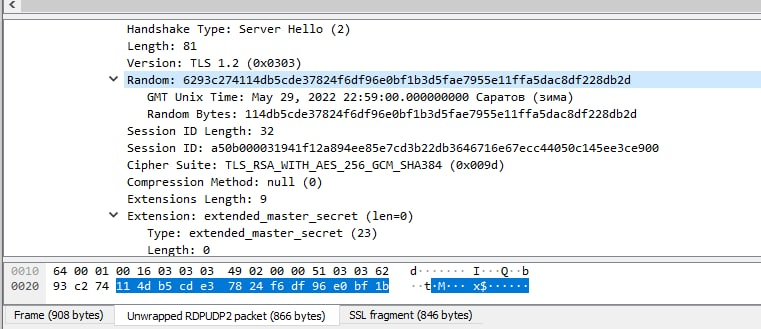
\includegraphics[width=0.9\textwidth]{photo/rndserv.png}
      \caption{Содержимое пакета, посылаемого от сервера клиенту (запись random сервера)}
      \label{rndserv}
    \end{figure}

    Совокупность открытого ключа и некоторая строка случайных байтов называется <<сертификатом>>. Данная запись изображена на рисунке \ref{cert}.
    
    \begin{figure}[H]
      \centering
      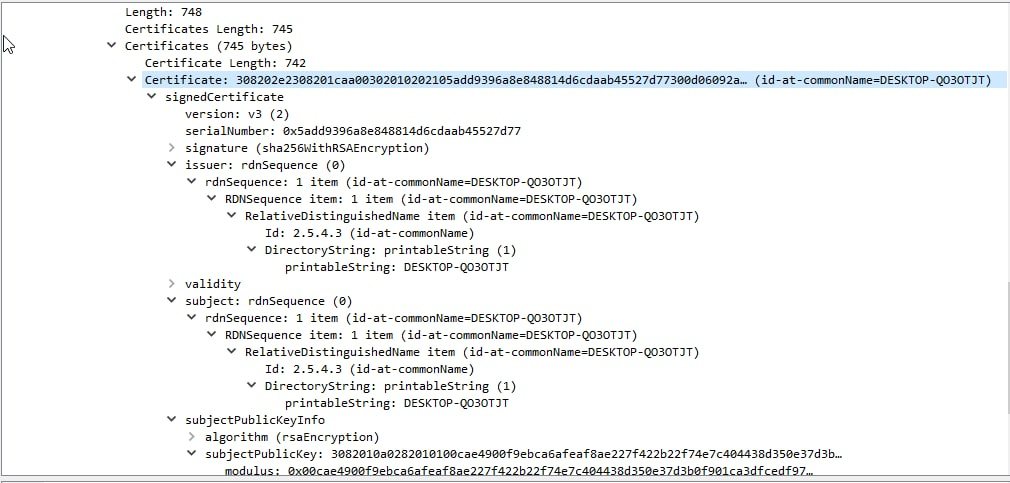
\includegraphics[width=0.9\textwidth]{photo/cert.png}
      \caption{Содержимое пакета, посылаемого от сервера клиенту (запись сертификата)}
      \label{cert}
    \end{figure}
    
    Сертификат подписывается службой терминалов, например, RDS, с использованием закрытого ключа для обеспечения подлинности.

    \item Теперь клиент посылает некоторую строку случайных байтов, которая называется <<premaster secret>>, показанная на рисунке \ref{cert1}. 
    
    \begin{figure}[H]
      \centering
      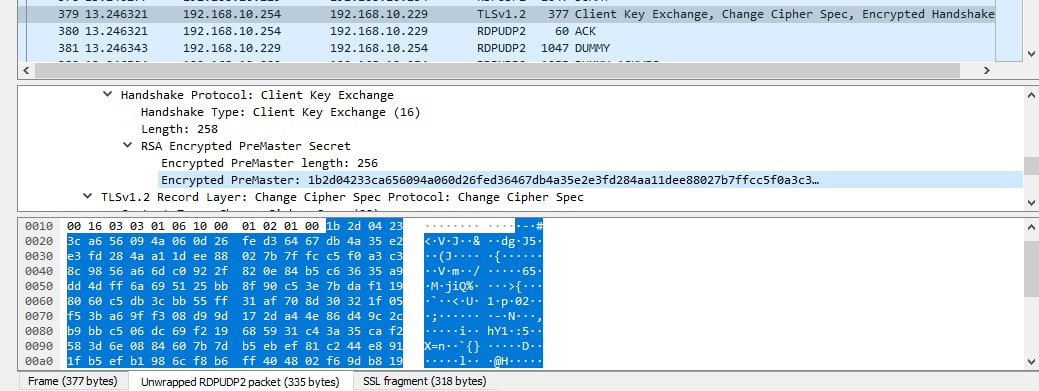
\includegraphics[width=0.9\textwidth]{photo/cert1.png}
      \caption{Содержимое пакета, посылаемого от клиента серверу (запись premaster secret)}
      \label{cert1}
    \end{figure}
    
    Данная запись шифруется открытым ключом, которая может быть расшифрована сервером только с помощью закрытого ключа службы терминалов.
    \item Сервер расшифровывает premaster secret с помощью собственного закрытого ключа.
    \item В случае успеха клиент и сервер получают свои сеансовые ключи из random сервера и premaster secret. Далее они используются для симметричного 
    шифрования остальной части сеанса.
  \end{enumerate}
  
  После того, как всё настроено, сессия RDP готова к работе. На ПК клиента от сервера поступает графическое изображение
  (результат операций), которое происходит в результате отправки команд с клавиатуры или мыши. Осталось только понять, как обнаружить передачу информации,
  характерную для подключения к удаленному рабочему столу.

  \section{Обнаружение сеанса удаленного управления с помощью программы}
  
  Одним из методов выявления сообщений, передаваемых по сети, является сниффер --- это программное обеспечение, которое анализирует входящий
  и исходящий трафик с компьютера, подключенного к интернету. Для данной работы была написана на языке Python программа <<sniffer.py>>, перехватывающая
  трафик сети.
    
  Данный сниффер принимает пакеты четвертой версии интернет-протоко- \\* ла, пакеты IPv4, содержащие в поле данных сообщения протоколов
  других уровней. В этом случае здесь будут рассматриваться сообщения протоколов транспортного уровня, а именно TCP- и UDP-протоколы.
    
  Для успешного перехвата трафика, необходимо установить неразборчивый режим на сетевой интерфейс, чтобы сетевая плата принимала
  все пакеты независимо от того, кому они адресованы. Данный выбор зависит от способа подключения устройства к сети. Например, в Linux
  есть виртуальный интерфейс (<<lo>>), который ваш компьютер использует для связи с самим собой, также существуют интерфейсы, относящиеся
  к проводному соединению (<<enp0s3>>) и беспроводному (<<wlp2s0>>). В данном случае все устройства будут подключены к сети через Ethernet.
  
  После выбора сетевого интерфейса сниффер начнет перехватывать трафик, как показано. В этот момент информация о перехваченных пакетах будет отображаться
  в консоли, а также будет записываться необходимая информация каждого пакета для анализа в текстовый файл.
  В результате работы программы <<sniffer.py>> будет получен файл data.log. Для обработки содержимого данного файла была написана программа
  <<data-analysis>>, реализованная также на языке Python. С помощью нее можно проанализировать весь перехваченный трафик относительно каждого
  IP-адреса, полученного из файла. Описание этих программ будет представлено ниже. 

  \subsection{Описание функций программы <<sniffer.py>>}

    Для анализа трафика в сети был создан сокет --- программный интерфейс для обеспечения обмена данными между процессами. В силу заданных параметров он
    получал пакеты, представленные в виде некоторой последовательности чисел, записанных в шестнадцатеричной системе счисления.
    
    % \begin{minted}[fontsize=\footnotesize]{Python}
    %   s_listen = socket.socket(socket.AF_PACKET, socket.SOCK_RAW, socket.ntohs(3))
    % \end{minted}
    
    Чтобы раскодировать данную последовательность чисел, необходимо обратиться к структуре пакета. Для начала нужно рассмотреть кадр Ethernet, представленный
    на рисунке \ref{eth-frame}.
    
    \begin{figure}[H]
      \centering
      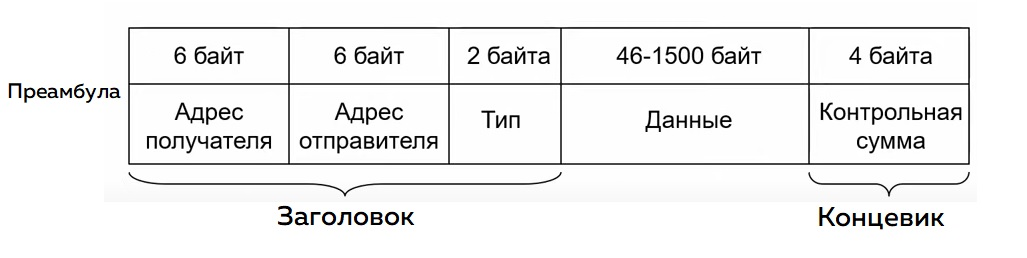
\includegraphics[width=0.9\textwidth]{photo/eth-frame.jpg}
      \caption{Структура Ethernet кадра}
      \label{eth-frame}
    \end{figure}
    
    Стоит отметить, что в данном заголовке нужно раскодировать 14 байт, 12 из которых MAC-адреса получателя и отправителя и 2 байта, идентифицирующие протокол
    сетевого уровня. К примеру, 0x0800 -- IPv4, 0x86DD -- IPv6 и т.д. С помощью функций \textit{get\_ethernet\_frame} и \textit{get\_mac\_addr} производится получение всех необходимых
    данных заголовка Ethernet.
    
    % \begin{minted}[fontsize=\footnotesize]{Python}
    %   # Получение ethernet-кадра
    %   def get_ethernet_frame(data):
    %     dest_mac, src_mac, proto = struct.unpack('!6s6sH', data[:14])
    %     return get_mac_addr(dest_mac), get_mac_addr(src_mac), socket.htons(proto)
      
      
    %   # Получение MAC-адреса
    %     def get_mac_addr(mac_bytes):
    %       mac_str = ''
    %       for el in mac_bytes:
    %         mac_str += format(el, '02x').upper() + ':'
    %       return mac_str[:len(mac_str) - 1]
    %   \end{minted}

    После получения информации об Ethernet кадре идет раскодирование интернет-протокола. В данной работе будут рассматриваться пакеты протокола IPv4, 
    так как для анализа данных этого вполне достаточно. Поэтому необходимо рассмотреть IPv4-заголовок, который показан на рисунке \ref{ipv4-header}.

    \begin{figure}[H]
      \centering
      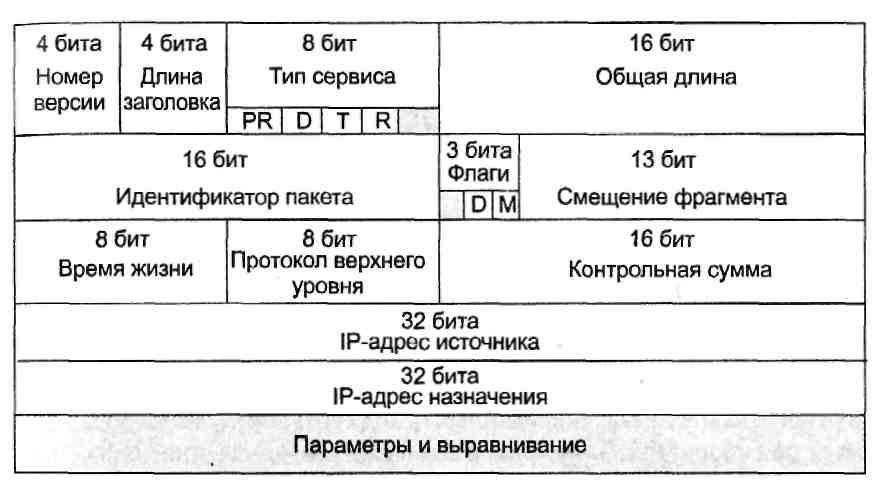
\includegraphics[width=0.9\textwidth]{photo/ipv4-header.jpg}
      \caption{Структура IPv4-заголовка}
      \label{ipv4-header}
    \end{figure}
      
    Обычно длина заголовка IP равна 20 байт, т.е. пять 32-битных слов, однако при увеличении объема служебной информации эта длина может быть увеличена
    за счет использования дополнительных байт в поле параметров и выравниваний. Благодаря полю, где содержится
    длина заголовка, можно правильно раскодировать оставшуюся последовательность байт. С помощью функций \textit{get\_ipv4\_data} и \textit{ipv4\_dec}
    будут получена информация о времени жизни текущего пакета, о номере транспортного протокола, об IP-адресах отправителя и получателя.
  
    % \begin{minted}[fontsize=\footnotesize]{Python}
    %   # Получение IPv4-заголовка
    %   def get_ipv4_data(data):
    %     version_header_length = data[0]
    %     header_length = (version_header_length & 15) * 4
    %     ttl, proto, src, dest = struct.unpack('!8xBB2x4s4s', data[:20])
    %     return str(ttl), proto, ipv4_dec(src), ipv4_dec(dest), data[header_length:]
      
      
    %   # Получение IP-адреса формата X.X.X.X
    %   def ipv4_dec(ip_bytes):
    %     ip_str = ''
    %     for el in ip_bytes:
    %       ip_str += str(el) + '.'
    %     return ip_str[:-1]
      
    % \end{minted}

    После того, как был получен номер транспортного протокола, можно раскодировать их данные. Как уже упоминалось ранее,
    в качестве транспортных протоколов будут рассматриваться TCP и UDP протоколы. На рисунке \ref{tcp-header} изображена структура TCP-заголовка.
  
    \begin{figure}[H]
      \centering
      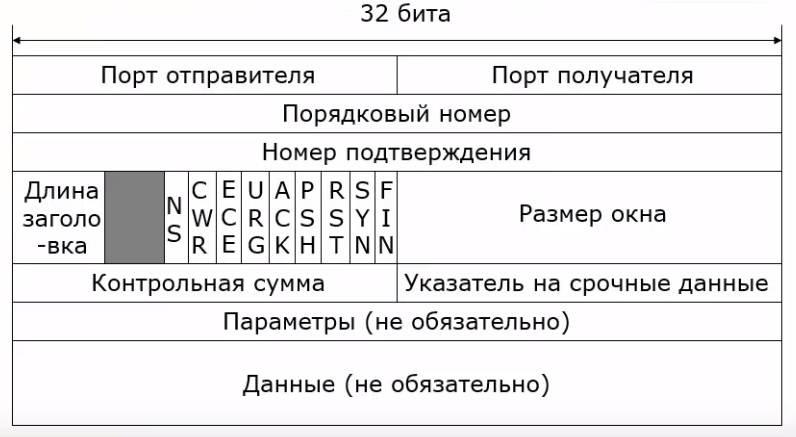
\includegraphics[width=0.9\textwidth]{photo/tcp-segment.jpg}
      \caption{Структура TCP-заголовка}
      \label{tcp-header}
    \end{figure}
    
    С помощью функции \textit{get\_tcp\_segment} производится получение информации, содержащейся в TCP-протоколе. Получается,
    теперь программе известны порт получателя, порт отправителя, порядковый номер, номер подтверждения, флаги и данные, которые
    содержат в себе TCP-заголовок.

    % \begin{minted}[fontsize=\footnotesize]{Python}
    %   # Получение TCP-cегмента данных
    %   def get_tcp_segment(data):
    %     src_port, dest_port, sequence, ack, some_block = struct.unpack('!HHLLH', data[:14])
    %     return str(src_port), str(dest_port), str(sequence), str(ack), \
    %            some_block, data[(some_block >> 12) * 4:]
    
    % \end{minted}

   Аналогично получается раскодирование данных UDP-заголовка с помощью функции \textit{get\_udp\_segment}.

    % \begin{minted}[fontsize=\footnotesize]{Python}
    %   # Получение UDP-сегмента данных
    %   def get_udp_segment(data):
    %     src_port, dest_port, size = struct.unpack('!HH2xH', data[:8])
    %     return str(src_port), str(dest_port), str(size), data[8:]
    % \end{minted}      

    Вся необходимая информация о пакетах для дальнейшего анализа записывается в файл data.log с помощью функции \textit{write\_to\_file}.
    
    % \begin{minted}[fontsize=\footnotesize]{Python}
    %   # Запись в файл
    %   def write_to_file(a):
    %     try:
    %       with open('data.log', 'a') as f:
    %         if a[5] == 'TCP':
    %           f.write( 'No:' + a[0] + ';' + 'Time:' + a[1] + ';' +
    %                    'Pac-size:' + a[2] + ';' + 'MAC-src:' + a[3] + ';' + 
    %                    'MAC-dest:' + a[4] + ';' + 'Type:' + a[5] + ';' +
    %                    'IP-src:' + a[6] + ';' + 'IP-dest:' + a[7] + ';' +
    %                    'Port-src:' + a[8] + ';' + 'Port-dest:' + a[9] + ';' +
    %                    'Seq:' + a[10] + ';' + 'Ack:' + a[11] + ';' +
    %                    'Fl-ack:' + a[12] + ';' + 'Fl-psh:' + a[13] + ';' +
    %                    'Fl-syn:' + a[14] + ';' + 'Len-data:' + a[15] + ';' + 
    %                    'Data:' + a[16] + ';!\n') 
    %         else:
    %           f.write( 'No:' + a[0] + ';' + 'Time:' + a[1] + ';' +
    %                    'Pac-size:' + a[2] + ';' + 'MAC-src:' + a[3] + ';' + 
    %                    'MAC-dest:' + a[4] + ';' + 'Type:' + a[5] + ';' +
    %                    'IP-src:' + a[6] + ';' + 'IP-dest:' + a[7] + ';' +
    %                    'Port-src:' + a[8] + ';' + 'Port-dest:' + a[9] + ';' +
    %                    'Len-data:' + a[10] + ';' + 'Data:' + a[11] + ';!\n')
    %         f.close()
    %     except:
    %       print('Ошибка записи в файл...')
    %       pass
    % \end{minted}


    Практически все выше перечисленные функции вызываются в \\* \textit{start\_to\_listen}, где осуществляется сбор информации
    о получаемых пакетах и вывод ее в консоль. Стоит отметить, что все выше описанные функции приведены в приложении А, где
    показан непосредственно сам код программы <<sniffer.py>>. Соответственно код программы <<data-analysis.py>> представлен в приложении Б.

  \subsection{Описание функций программы <<data-analysis.py>>}

  При запуске программа попросит пользователя ввести название файла. Далее производится считывание файла с помощью функции \textit{read\_from\_file},
  где в это время сохраняется информация о каждом пакете, перехваченном во время работы программы <<sniffer.py>>.

  % \begin{minted}[fontsize=\footnotesize]{Python}
  %   # Считывание с файла и заполнение массива
  %   # Packet_list объектами класса PacketInf
  %   def read_from_file(inf):
  %     a = []
  %     while True:
  %       beg = inf.find(':')
  %       end = inf.find(';')
  %       if beg == -1 and end == -1:
  %         break
  %       else:
  %         a.append(inf[beg + 1: end])
  %       inf = inf[end + 1:]
  %     try:
  %       if a[5] == 'TCP':
  %         Packet_list.append(PacketInf( a[0], a[1], a[2], a[3], a[4], a[5]
  %                                     , a[6], a[7], a[8], a[9], a[15], a[16]
  %                                     , a[10], a[11], a[12], a[13], a[14] ))
  %       elif a[5] == 'UDP':
  %         Packet_list.append(PacketInf( a[0], a[1], a[2], a[3], a[4], a[5]
  %                                     , a[6], a[7], a[8], a[9], a[10], a[11] ))
  %     except:
  %       print('Ошибка при считывании файла...')
  %       exit(0)
  % \end{minted}

  После считывания собирается некоторая общая информация о перехваченном трафике. Под общей информацией подразумевается: время начала и завершения
  перехвата трафика, количество пакетов, среднее количество пакетов в секунду, средний размер пакетов. Вместе с этим в консоль выводится список 
  IP-адресов, участвующих в передаче пакетов по сети, в момент работы программы <<sniffer.py>>. Пользователю предоставляется возможность выбрать
  интересующий его IP-адрес для дальнейшего анализа пакетов, связанных с ним. После выбора конкретного IP-адреса осуществляется вывод опять же общей
  информации, но уже только относительно выбранного IP-адреса. Т.е. выводится время первого и последнего перехваченных пакетов, где в качестве отправителя
  или получателя выступает данный IP-адрес. 
  
  Таким образом можно понять, в какой конкретно момент времени начался обмен информацией с тем или иным 
  IP-адресом. Также рассчитываются количество пакетов, среднее количество пакетов в секунду и средний размер пакетов для определения общего объема 
  информации, передаваемой в данный отрезок времени. Помимо этого, пользователю предоставляются некоторые опции, которые будут описаны ниже:
  
  \begin{enumerate}
    \item Пользователю предоставляется возможность вывести весь сетевой трафик, где в качестве отправителя или получателя выступает выбранный IP-адрес.
    \item При выборе второй опции строится график отношения входящего и исходящего трафиков в единицу времени. Данное отношение рассчитывается по формуле
    
    \begin{center}
      $r_{ip} = \frac{V_{dest}}{V_{src}}$,
    \end{center}

    где $V_{dest}$ и $V_{src}$ --- объемы соответственно входящего и исходящего трафика в единицу времени. 
    % Значениям оси абсцисс будут соответствовать
    % секунды, которые будут отсчитываться с момента начала работы программы. Значениям оси ординат, рассчитанные по приведенной выше формуле, будут
    % соответвовать каждому такому значению $x$. 
     
    При большой величине входящего трафика, можно узнать в какой момент времени происходит обмен информацией с каким-либо другим IP-адресом.
    \item При выборе третьей опции строится график отношения $V_{udp}$ --- объема входящего UDP-трафика и $V_{tcp}$ объема входящего TCP-трафика.
    Отношение рассчитывается по формуле

    \begin{center}
      $r_{udp} = \frac{V_{udp}}{V_{tcp}}$.
    \end{center}

    Так как во время RDP-сессии осуществляется передача пакетов по протоколу UDP и TCP, то анализируя полученную информацию исходя из этого графика,
    можно установить признаки RDP-сессии.

    \item При выборе данной опции строится график разности количества исходящих и входящих TCP-пакетов, в которых флаг ACK имеет значение
    равное единице.

    \begin{center}
      $r_{ack} = V_{A_{out}} - V_{A_{in}}$,
    \end{center}

    где $V_{A_{in}}$ и $V_{A_{out}}$ --- число входящих и исходящих ACK-флагов в TCP-трафике в единицу времени. При подключении к удаленному рабочему 
    столу сервер отправляет клиенту TCP-пакеты с установленным флагом ACK, указывающим, что поле номера подтверждения задействовано. В таком случае с
    помощью графика можно определить клиента и сервер.
    \item При выборе пятой опции строятся два графика, показывающие частоту SYN-флагов и PSH-флагов в TCP-трафике. Частота SYN-флагов находится по формуле
    
    \begin{center}
      $r_{syn} = \frac{V_{S_{in}}}{V_{tcp}}$,
    \end{center}

    где $V_{S_{in}}$ число входящих TCP-пакетов, в которых установлен флаг SYN = 1, $V_{tcp}$ --- число входящих TCP-пакетов в единицу времени.
    SYN-флаг служит для синхронизации номеров сессии приема или передачи данных.

    Частота PSH-флагов вычисляется по формуле 
    
    \begin{center}
      $r_{psh} = \frac{V_{P_{in}}}{V_{tcp}}$,
    \end{center}
    
    где $V_{P_{in}}$ число входящих TCP-пакетов, в которых установлен флаг PSH = 1, $V_{tcp}$ --- число входящих TCP-пакетов в единицу времени.
    PSH-флаг инструктирует получателя, чтобы он отправил накопившиеся в приемном буфере данные в приложение отправителя.
  \end{enumerate}

  После описания всех опций данной программы остается только показать, как это будет выглядеть на практике.

  \section{Демонстрация работы программ}

  Для тестирования данных программ было запущено три виртуальных машины. Две из них (ПК-1 и ПК-2) имеют операционную систему Windows 10 Professional версии 21H2.
  И у одной машины (ПК-3) поставлена операционная система Linux Ubuntu 22.04 LTS. Все устройства не имеют доступа к интернету, однако каждая виртуальная машина 
  может взаимодействовать друг с другом.

  Запустив программу <<sniffer.py>>, был произведен захват трафика, как показано на рисунке \ref{cmd-strt}.
  
  \begin{figure}[H]
    \centering
    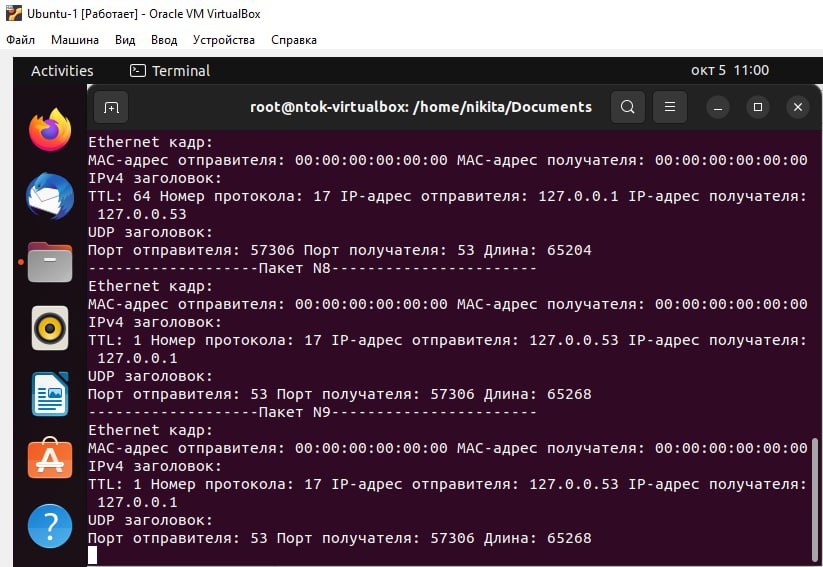
\includegraphics[width=0.9\textwidth]{photo/cmd-start.jpg}
    \caption{Вид консоли при работе программы <<sniffer.py>>}
    \label{cmd-strt}
  \end{figure}
  
  Во время работы программы совершались следующие действия:

  \begin{enumerate}
    \item В 12:03 на ПК2 была запущена программа <<Подключение к удаленному рабочему столу>>.
    \item Примерно через 15 секунд было совершено подключение ПК2 к ПК1 по протоколу RDP.
    \item Начиная с 12:03:50 производилось движение мышкой по рабочему столу, открытие текстовых файлов, лежащих на рабочем 
    столе ПК1.
    \item В 12:04:51 было завершено подключение к удаленному рабочему столу ПК1.
  \end{enumerate}
  
  После завершения программы <<sniffer.py>> был получен файл data.log, в котором хранится вся необходимая информация о каждом перехваченном пакете.
  Запустив программу <<data-analysis.py>> и введя название анализируемого файла, в консоли отображается общие сведения о перехваченном трафике, как показано
  на рисунке \ref{cmd-strt2}.
  
  \begin{figure}[H]
    \centering
    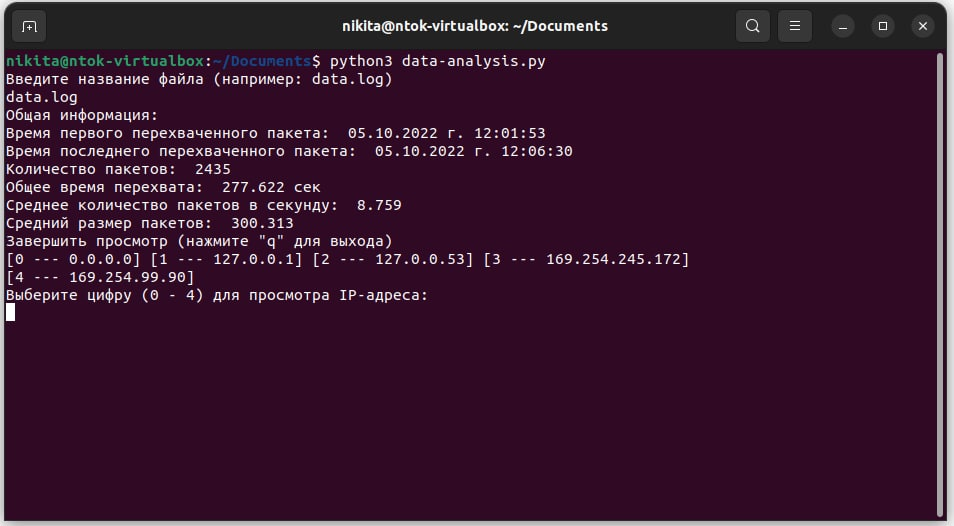
\includegraphics[width=0.9\textwidth]{photo/cmd-start2.jpg}
    \caption{Вид консоли при работе программы <<data-analysis.py>>}
    \label{cmd-strt2}
  \end{figure}

  Из рисунка \ref{cmd-strt2} видно, что в данном промежутке времени в обмене данными принимали участие всего 5 IP-адресов, первые три из которых рассылает
  устройство ПК3. А последние два принадлежат ПК1 и ПК2. Осталось только определить какой IP-адрес принадлежит серверу, а какой --- клиенту. Конечно, больше
  всего сейчас интересны последние два IP-адреса, поэтому далее пользователь введет значение 3, чтобы выбрать IP-адрес 169.254.245.172.

  На рисунке \ref{chmod} показана информация, связанная с IP-адресом 169.254.245.\\*172.

  \begin{figure}[H]
    \centering
    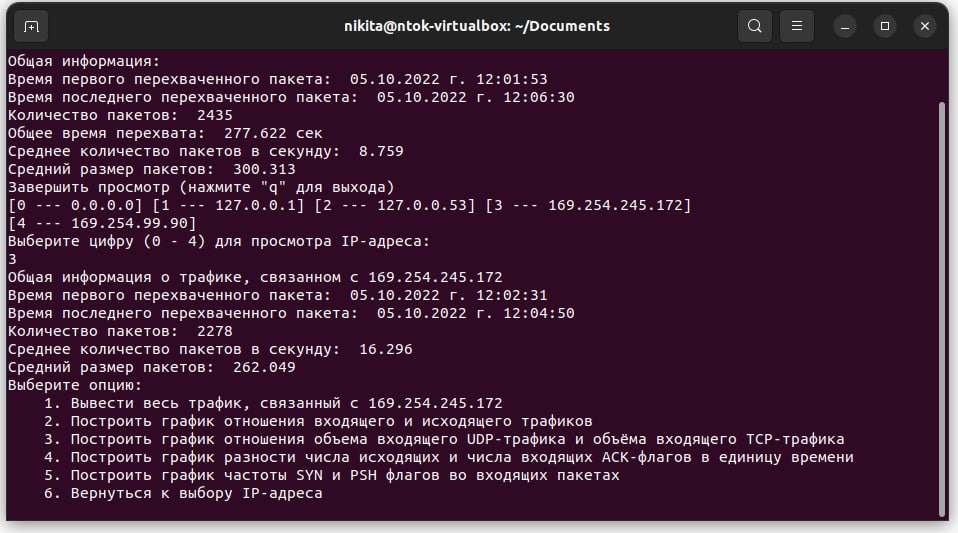
\includegraphics[width=0.9\textwidth]{photo/choose-mode.jpg}
    \caption{Вид консоли при выборе IP-адреса 169.254.245.172}
    \label{chmod}
  \end{figure}

  При выборе второй опции будет построен график, изображенный на рисунке \ref{clnt1}.

  \begin{figure}[H]
    \centering
    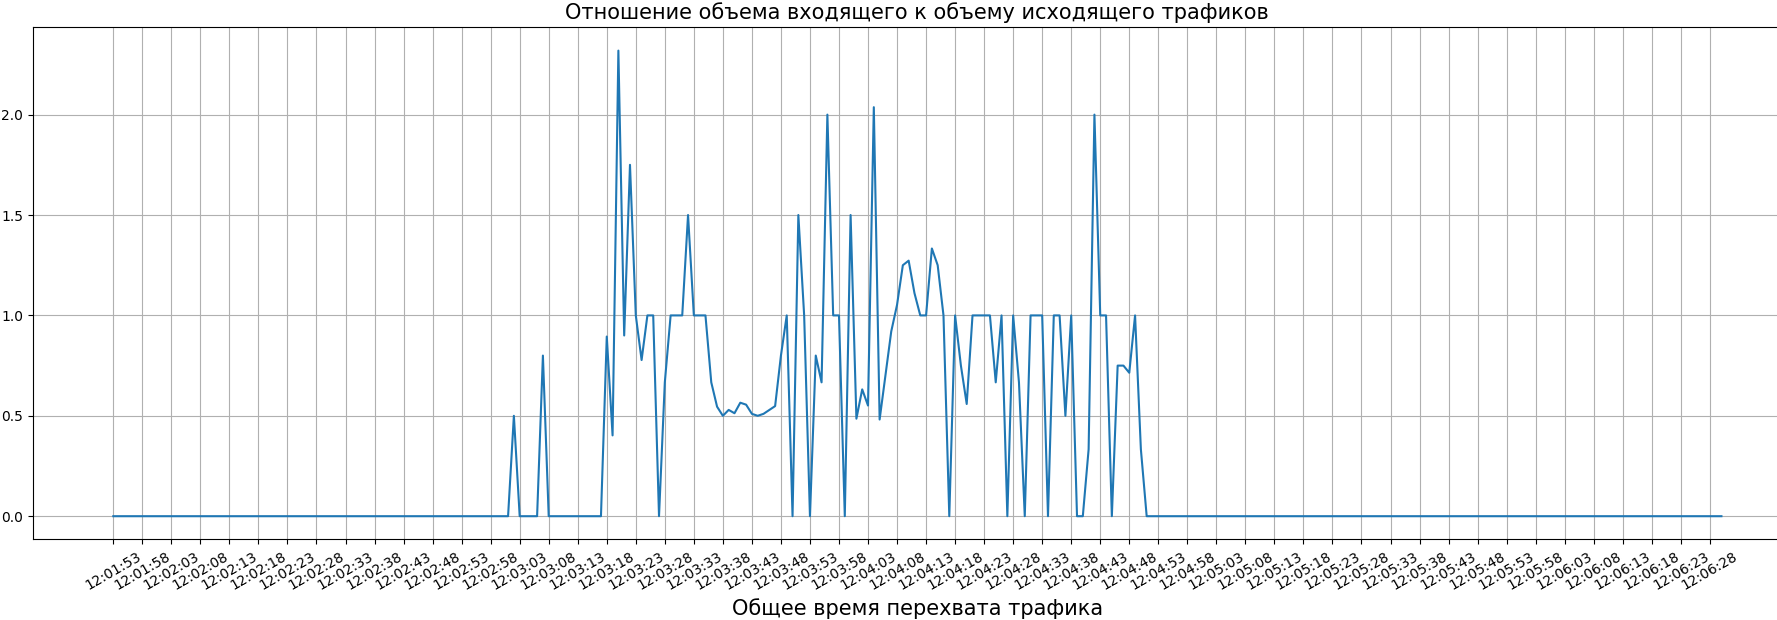
\includegraphics[width=0.9\textwidth]{photo/clnt1.png}
    \caption{График отношения входящего и исходящего трафиков относительно 169.254.245.172}
    \label{clnt1}
  \end{figure}

  Из рисунка \ref{clnt1} видно, что значение переменной $V_{dest}$ начинает возрастать с 12:03:18, а на 12:03:20 эта величина достигает
  своего максимального значения.

  Теперь для сравнения на следующем рисунке будет показан график отношения входящего и исходящего трафиков, но уже относительно IP-адреса 169.254.99.90.

  \begin{figure}[H]
    \centering
    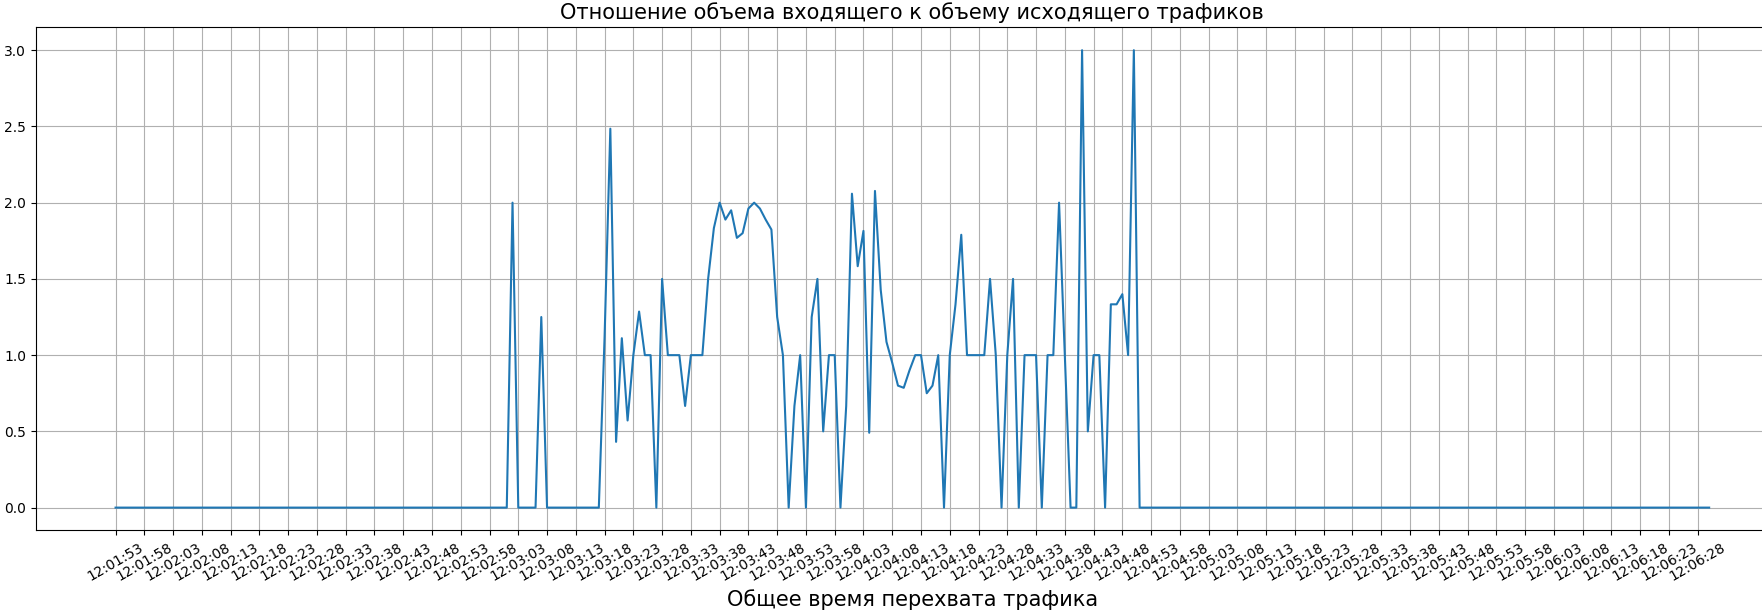
\includegraphics[width=0.9\textwidth]{photo/serv1.png}
    \caption{График отношения входящего и исходящего трафиков относительно 169.254.99.90}
    \label{serv1}
  \end{figure}

  Если посмотреть на следующий рисунок, то можно увидеть в данном трафике, что первый пакет был передан по порту 3389 в 12:03:02. Это также видно из
  графиков, показанных на рисунках \ref{clnt1} и \ref{serv1}. Тогда начиная с 12:03:18 произошла установка RDP-сессии.
  
  \begin{figure}[H]
    \centering
    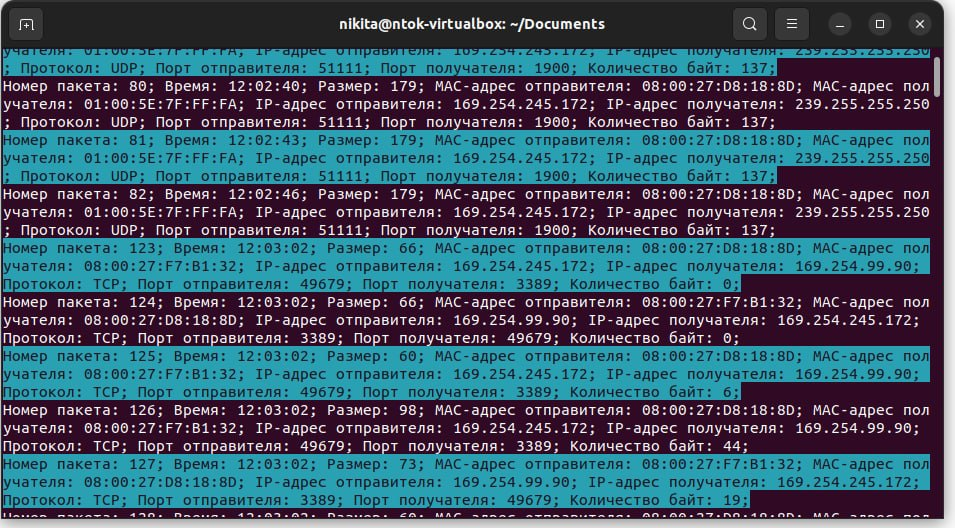
\includegraphics[width=0.9\textwidth]{photo/traffic-1.jpg}
    \caption{Просмотр трафика, связанного с 169.254.245.172}
    \label{traf1}
  \end{figure}
  
  Исходя из рисунков \ref{clnt2} и \ref{serv2}, можно сделать вывод, что в промежутке 12:03:18 -- 12:03:25 передается большой объем UDP-пакетов и 
  скорее всего это произошло в момент подтверждения сертификата клиента сервером.

  \begin{figure}[H]
    \centering
    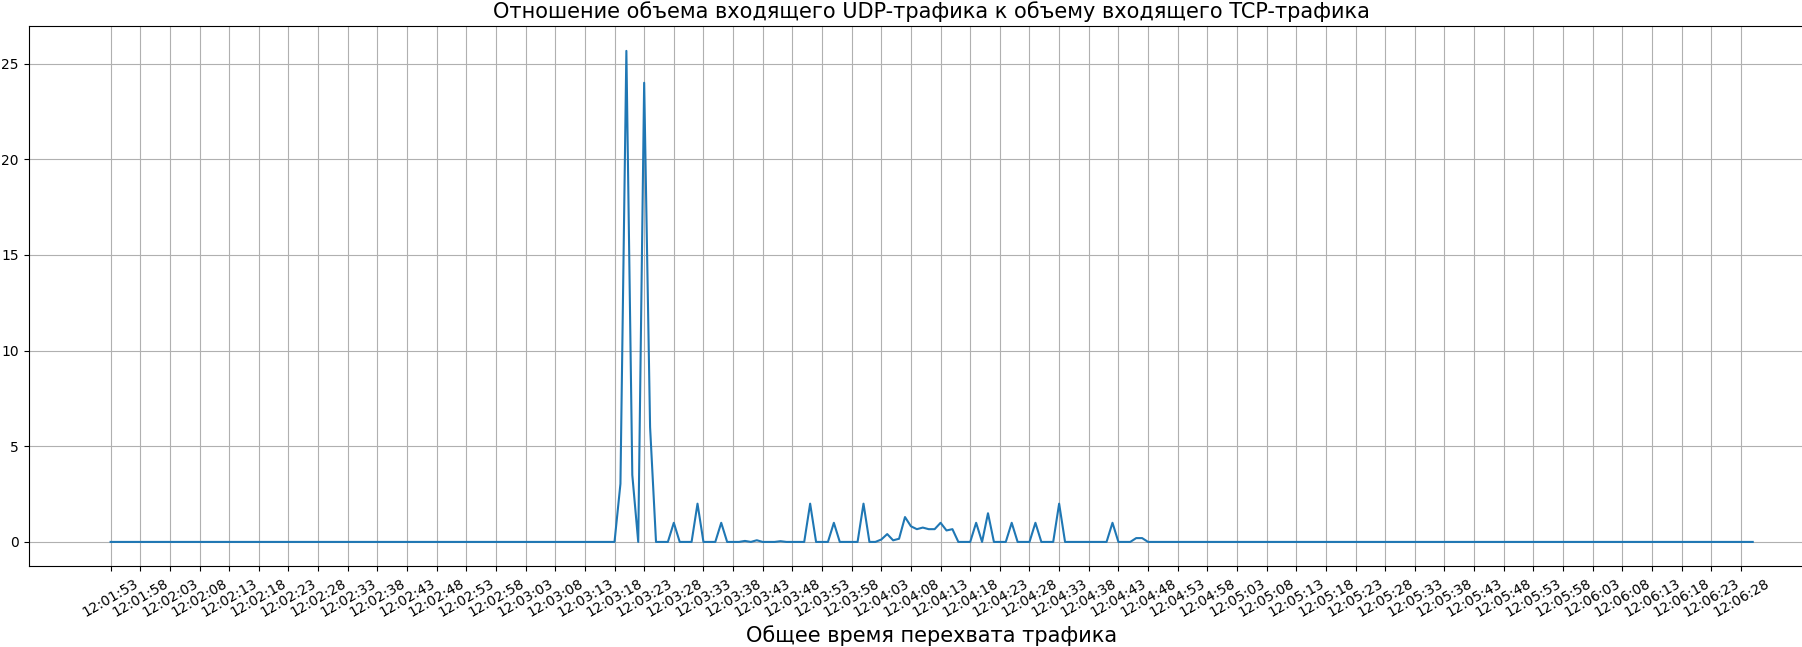
\includegraphics[width=0.9\textwidth]{photo/clnt2.png}
    \caption{График, построенный по формуле $r_{udp} = \frac{V_{udp}}{V_{tcp}}$ относительно 169.254.245.172}
    \label{clnt2}
  \end{figure}

  \begin{figure}[H]
    \centering
    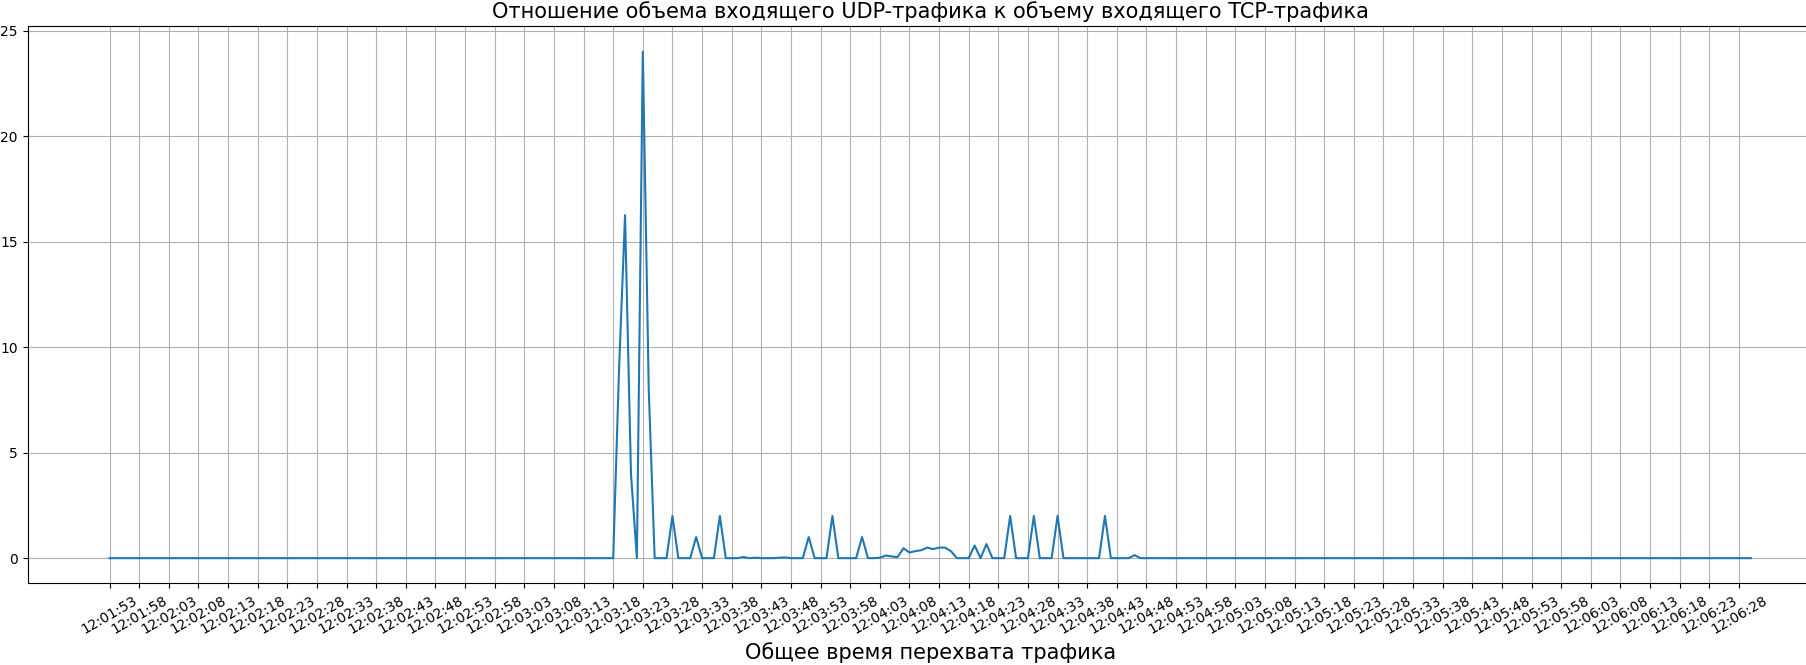
\includegraphics[width=0.9\textwidth]{photo/serv2.png}
    \caption{График, построенный по формуле $r_{udp} = \frac{V_{udp}}{V_{tcp}}$ относительно 169.254.99.90}
    \label{serv2}
  \end{figure}

  На рисунках \ref{clnt3} и \ref{serv3} изображены графики разности числа исходящих и входящих ACK-флагов в единицу времени.

  \begin{figure}[H]
    \centering
    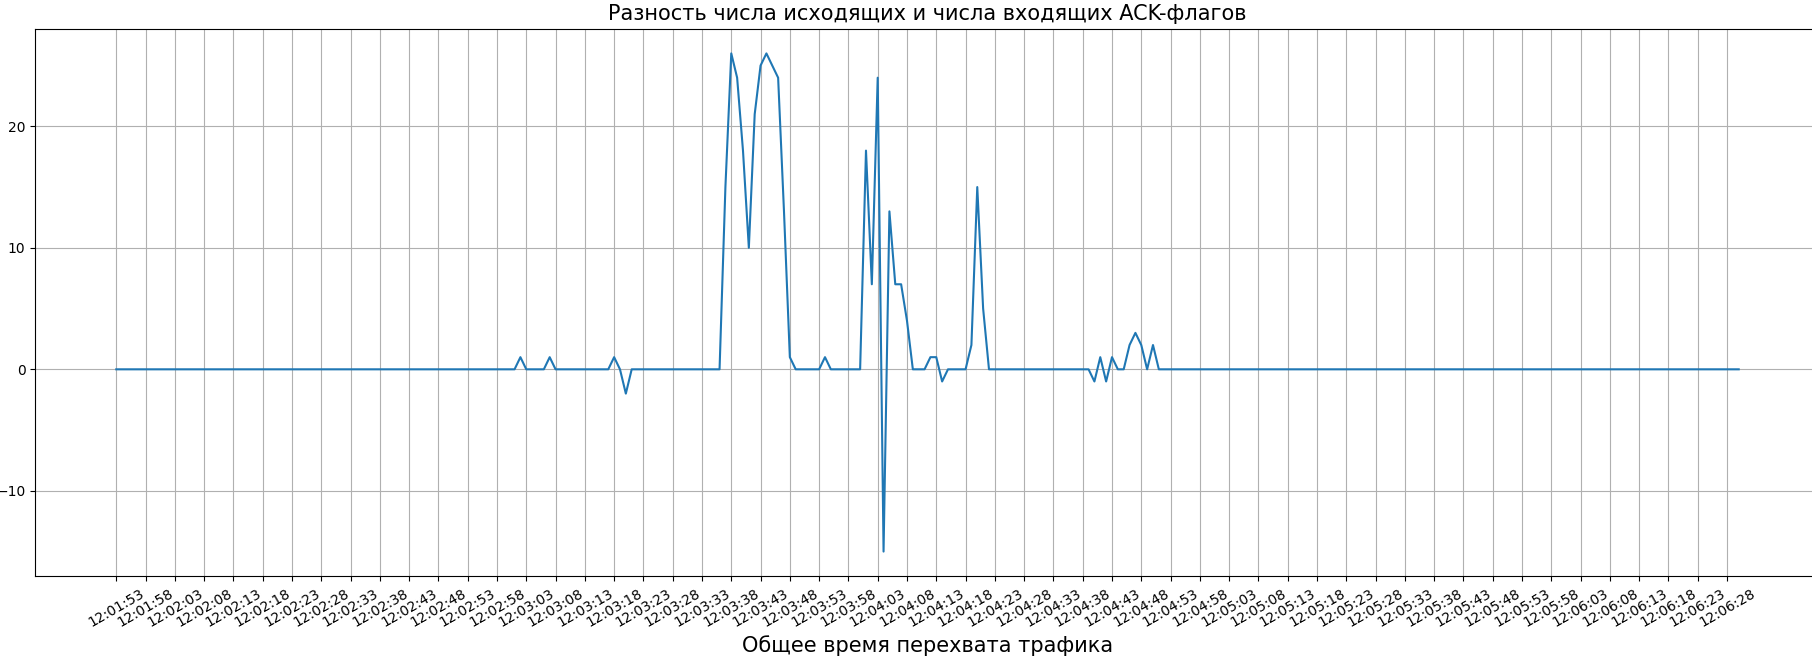
\includegraphics[width=0.9\textwidth]{photo/clnt3.png}
    \caption{График, построенный по формуле $r_{ack} = V_{A_{out}} - V_{A_{in}}$ относительно 169.254.245.172}
    \label{clnt3}
  \end{figure}

  Величина $V_{A_{in}}$ показывает, как часто сервер отказывает клиенту из-за перегрузки. На промежутке 12:03:36 -- 12:03:49 видно, что 
  осуществляется обмен данными между клиентом и сервером. Как показано на рисунке \ref{serv3} отрицательное значение объема $V_{A_{in}}$
  означает, что на данном промежутке времени сервер, получая от клиента TCP-пакеты с установленным ACK-флагом, теряет возможность
  отвечать на запросы клиента. 

  \begin{figure}[H]
    \centering
    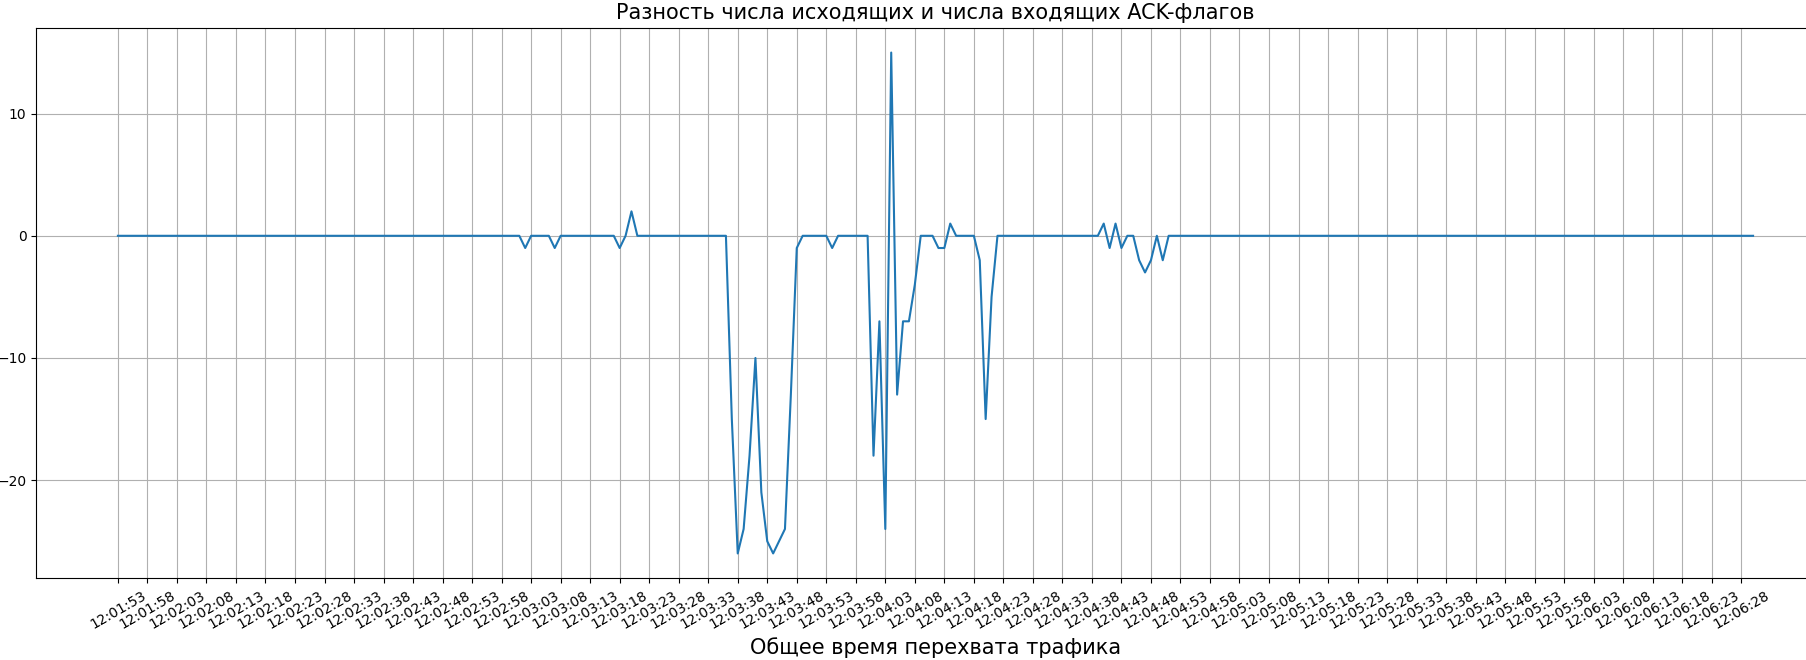
\includegraphics[width=0.9\textwidth]{photo/serv3.png}
    \caption{График, построенный по формуле $r_{ack} = V_{A_{out}} - V_{A_{in}}$ относительно 169.254.99.90}
    \label{serv3}
  \end{figure}

  Получается, что ПК1 (серверу) соответствует адрес 169.254.99.90, а ПК2 (клиенту) --- 169.254.245.172.

  На рисунках \ref{clnt4} и \ref{serv4} изображены графики частот SYN- и PSH-флагов.

  \begin{figure}[H]
    \centering
    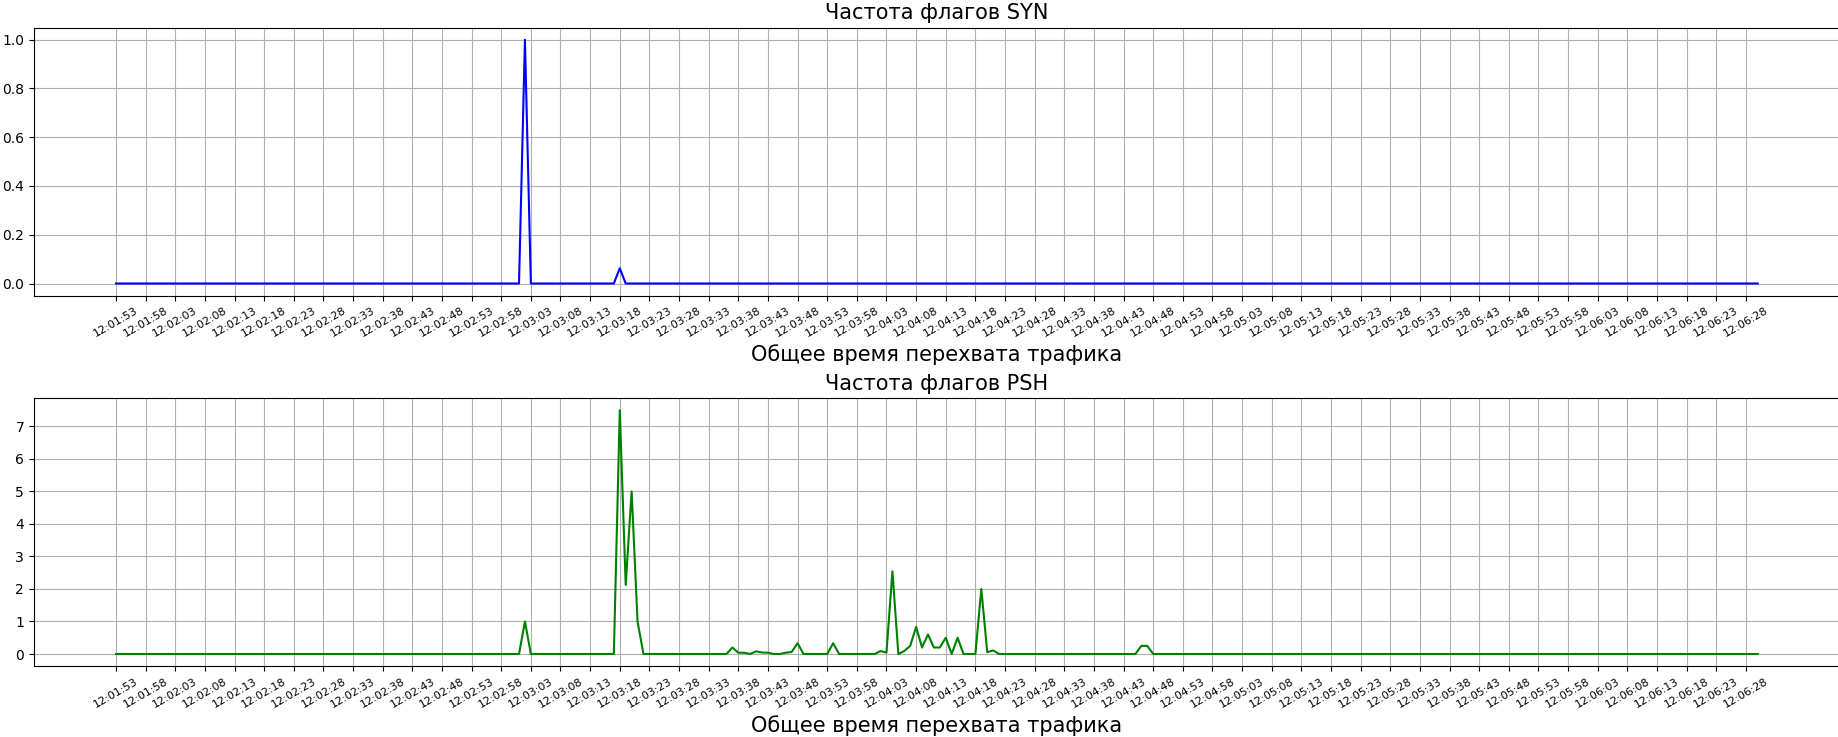
\includegraphics[width=0.9\textwidth]{photo/clnt4.png}
    \caption{График, построенный по формуле $r_{syn} = \frac{V_{S_{in}}}{V_{tcp}}$ относительно 169.254.245.172}
    \label{clnt4}
  \end{figure}

  \begin{figure}[H]
    \centering
    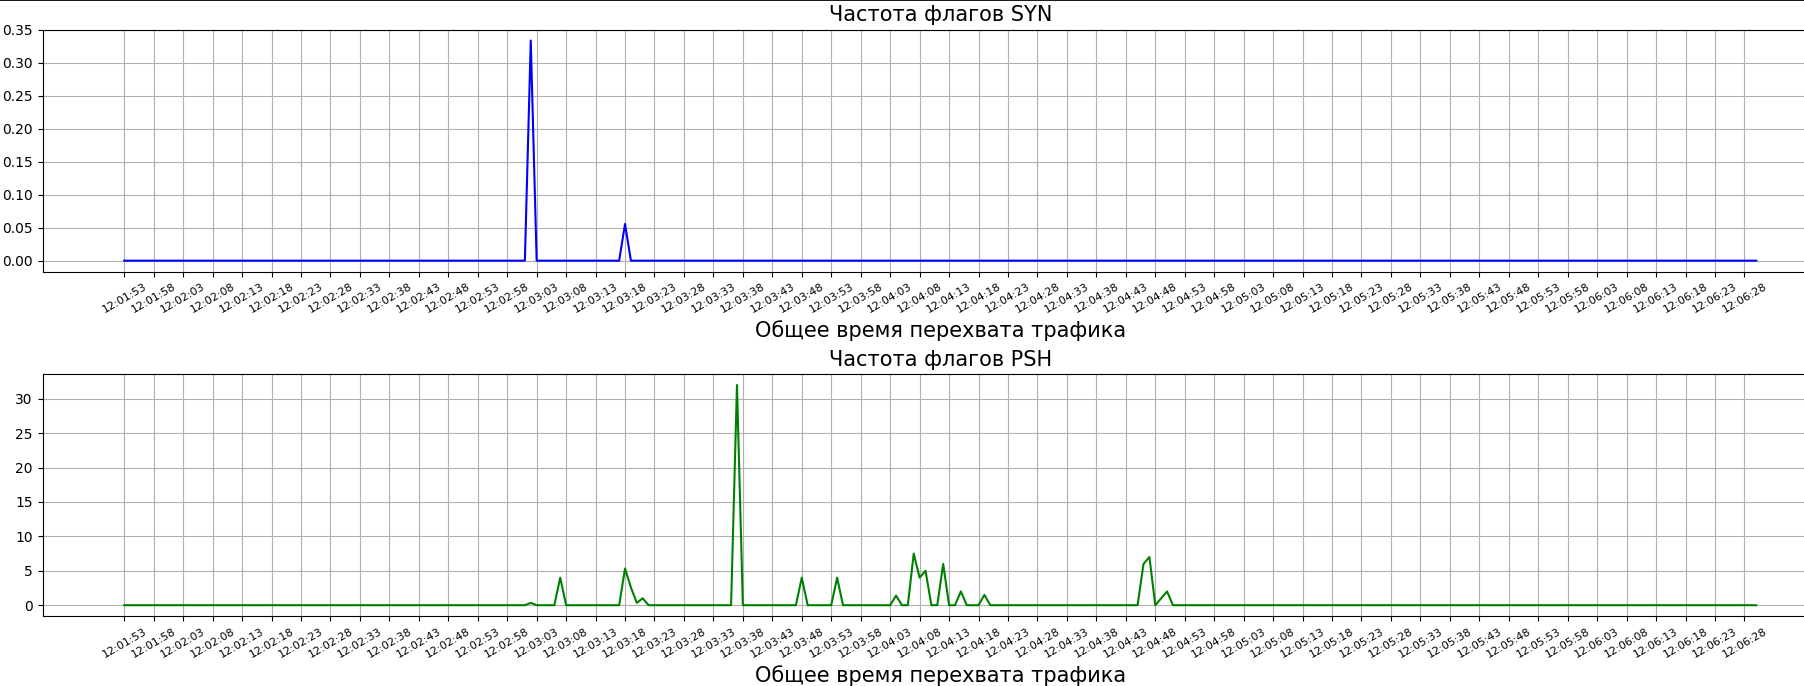
\includegraphics[width=0.9\textwidth]{photo/serv4.png}
    \caption{График, построенный по формуле $r_{psh} = \frac{V_{P_{in}}}{V_{tcp}}$ относительно 169.254.99.90}
    \label{serv4}
  \end{figure}

  Стоит отметить, что по последним двум графикам можно сделать вывод исходя из количества PSH-флагов в момент времени 12:03:17 --
  12:03:22, как показано на рисунке \ref{clnt4}. На этом отрезке времени передаются также TCP-пакеты с установленным PSH-флагом,
  сигнализируя протоколу TCP отправить все данные, независимо от того, где и сколько их было уже передано.

  По построенным графикам можно сделать несколько выводов.
  Например, из рисунка \ref{clnt2} отчетливо видно, что с 12:03:50 начинается рост значения $V_{udp}$, а значит
  увеличивается объем входящего UDP-трафика ПК2. Это можно аргументировать тем, что в этот момент времени происходят
  различные операции, сделанные на рабочем столе ПК1. В данном случае были произведены движения мышкой.

  Также из рисунков \ref{clnt1} и \ref{serv1} видно, что обмен данными между ПК1 и ПК2 прерывается в 12:04:51. Тогда можно
  предположить, что именно в это время закончилась RDP-сессия.
  
  
  \conclusion
  
  В результате проделанной работы были разобраны методы обнаружения подключения к удаленному рабочему столу по протоколу RDP, где с помощью различных программ
  удалось рассмотреть принцип работы RDP-протокола. Стоит отметить, что хоть RDP далеко не самый защищенный протокол, его обнаружение может стать затруднительным,
  особенно когда производится подключение к удаленному рабочему столу в реальных условиях с выходом в интернет. И для его анализа обычного перехвата трафика будет
  недостаточно. Однако, благодаря различным метрикам и построенным по ним графикам, по которым анализируют сетевые атаки, можно получить полезную информацию. 
  Поэтому в дальнейшем, опираясь на проделанную работу, будут совершены попытки выявления протокола RDP от всех прочих протоколов сети интернет 
  путем анализа данных по построенным графикам.
  

  \begin{thebibliography}{15}
    \bibitem{1}
    Книга Ибе О.С. «Компьютерные сети и службы удаленного доступа» / пер. с англ. -
    Москва, издательство: «ДМК Пресс», Яз. рус.
    \bibitem{2}
    Удалённый рабочий стол RDP: как включить и как подключиться по RDP [Электронный ресурс] / URL:https://hackware.ru/?p=11835 (дата обращения 03.05.2022), Яз. рус.
    \bibitem{userdp1}
    How to use remote desktop [Электронный ресурс] / URL: https://support.microsoft.com/en-us/windows/how-to-use-remote-desktop-5fe128d5-8fb1-7a23-3b8a-41e636865e8c (дата обращения 27.05.2022), Яз. англ.
    \bibitem{userdp2}
    Статья <<Как исправить ошибку удаленного рабочего стола не удается подключиться к удаленному компьютеру>> [Электронный ресурс] / URL: https://okdk.ru/kak-ispravit-oshibku-udalennogo-rabochego-stola-ne-udaetsya-podkljuchitsya-k-udalennomu-kompjuteru/ 
    (дата обращения 27.05.2022), Яз. рус.
    \bibitem{rdp2}
    Документация Remote Utilities <<RDP>> [Электронный ресурс] / URL:  https://www.remoteutilities.com/support/docs/rdp/ (дата обращения 27.05.2022), Яз. англ.
    % \bibitem{3}
    % Документация по устранению неполадок служб удаленных рабочих стола для Windows Server [Электронный ресурс] / URL: https://inlnk.ru/bvOV0 (дата обращения 04.05. 2022), Яз. рус.
    \bibitem{socket1}
    Документация по стандартным библиотекам языка Python [Электронный ресурс] / URL: https://docs.python.org/3/library/socket.html (дата обращения 25.06.2022), Яз. англ.
    \bibitem{socket2}
    Статья <<Интерактивная система просмотра системных руководств (man-ов)>> [Электронный ресурс] / URL: https://www.opennet.ru/cgi-bin/opennet/man.cgi?topic=socket\&category=2 (дата обращения 25.06.2022), Яз. англ.
    \bibitem{rdpudp}
    Документация Microsoft <<Протоколы>> [Электронный ресурс] / URL: https://docs.microsoft.com/en-us/openspecs/windows_protocols/ms-rdpeudp2/d8bf9a56-90f3-4608-8f98-9600ed69876b (дата обращения 28.05.2022), Яз. рус.
    \bibitem{rdp1}
    Статья <<Wireshark Tutorial: Decrypting RDP Traffic>> [Электронный ресурс] / URL: https://unit42-paloaltonetworks-com.translate.goog/wireshark-tutorial-decrypting-rdp-traffic/?_x_tr_sl=en\&_x_tr_tl=ru\&_x_tr_hl=ru\&_x_tr_pto=op,wapp
    (дата обращения 28.05.2022), Яз. англ.
    \bibitem{tcpflags}
    Статья <<TCP flags>> [Электронный ресурс] / URL: https://www.keycdn.com/support/tcp-flags\#:~:text=ACK
    (дата обращения 02.10.2022), Яз. англ.
  \end{thebibliography}

  \appendix

    \section{Код sniffer.py}
    \inputminted[fontsize=\footnotesize]{Python}{code/sniffer.py}


    \section{Код data-analysis.py}
    \inputminted[fontsize=\footnotesize]{Python}{code/data-analysis.py}
\end{document}